\documentclass[11pt]{article}

%%%%%%%%%%%%%%%%
% Handout vs. key
%%%%%%%%%%%%%%%%

%%% Handout
\newcommand{\soln}[2]{\vspace{#1}}{}
\newcommand{\solnMult}[1]{ #1 }
\newcommand{\tf}[1]{}

%% Key
%\newcommand{\soln}[2]{\textcolor{custom_darkBlue}{\textit{#2}}}{}
%\newcommand{\solnMult}[1]{\textbf{\textcolor{custom_darkBlue}{\textit{#1}}}}
%\newcommand{\tf}[1]{ \textbf{\textcolor{custom_darkBlue}{\textit{#1}}} }

%%%%%%%%%%%%%%%%
% Packages
%%%%%%%%%%%%%%%%

\usepackage[top=2cm,bottom=2cm,left=1.5cm,right= 1.5cm]{geometry}
\usepackage[parfill]{parskip}
\usepackage{graphicx, xcolor,multicol, enumerate, setspace, changepage, amsmath}
\DeclareGraphicsRule{.tif}{png}{.png}{`convert #1 `dirname #1`/`basename #1 .tif`.png}

%%%%%%%%%%%%%%%%
% Header
%%%%%%%%%%%%%%%%

\usepackage{fancyhdr}
\pagestyle{fancy}

\lhead{\textcolor{custom_blue}{{\sc Dr. \c{C}etinkaya-Rundel}}}
\rhead{\textcolor{custom_blue}{{\sc Sta 101 - DASI}}}
\chead{\textcolor{custom_blue}{{\sc Sample Midterm 1}}}

%%%%%%%%%%%%%%%%
% User defined colors
%%%%%%%%%%%%%%%%

% Pantone 2015 Spring colors
% http://iwork3.us/2014/09/16/pantone-2015-spring-fashion-report/
% update each semester or year

\xdefinecolor{custom_blue}{rgb}{0, 0.70, 0.79} % scuba blue
\xdefinecolor{custom_darkBlue}{rgb}{0.11, 0.31, 0.54} % classic blue
\xdefinecolor{custom_orange}{rgb}{0.97, 0.57, 0.34} % tangerine
\xdefinecolor{custom_green}{rgb}{0.49, 0.81, 0.71} % lucite green
\xdefinecolor{custom_red}{rgb}{0.58, 0.32, 0.32} % marsala

\xdefinecolor{custom_lightGray}{rgb}{0.78, 0.80, 0.80} % glacier gray
\xdefinecolor{custom_darkGray}{rgb}{0.54, 0.52, 0.53} % titanium

%%%%%%%%%%%%%%%%
% Custom commands
%%%%%%%%%%%%%%%%

\newenvironment{choices}{
\begin{enumerate}[(a)]
}{\end{enumerate}}

\newcommand{\qt}[1]{\textcolor{custom_blue}{\textbf{\textit{#1.}}}}

\renewcommand{\emph}[1]{\underline{\textbf{#1}}}

%%%%%%%%%%%%%%%%
% Begin document
%%%%%%%%%%%%%%%%

\begin{document}

%%%%%%%%%%%%%%%%%%%%%%%%%%%%%%%%%%%%%%%

\begin{enumerate}

%%%%%%%%%%%%%%%%%%%%%%%%%%%%%%%%%%%%%%%

\item \qt{Reaction distance} Reaction distances (in centimeters) for the dominant hand were recorded from a random sample of 40 randomly chosen college students. Smaller distances indicate quicker reactions. A box plot of the distribution as well as summary statistics are provided below. A professor claims that college students have \emph{quicker} reactions than the general population. The overall mean for the general population is 10 centimeters. \\

\begin{center}
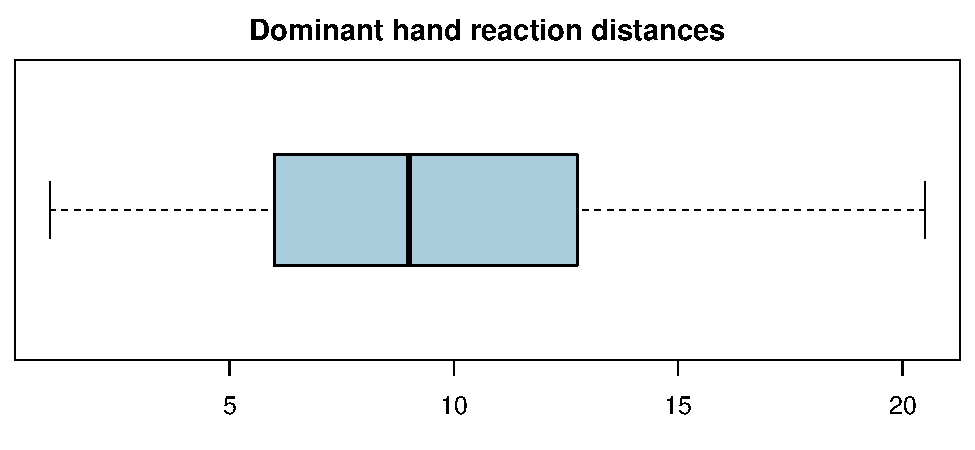
\includegraphics[width=0.6\textwidth]{figures/reaction_times/reaction_times_boxplot}
\renewcommand{\arraystretch}{2}
\begin{tabular}{c|c|c|c|c|c|c|c}
Min. 	& 1st Qu.	& Median	& Mean	& 3rd Qu.	& Max.	& SD		& n  \\
\hline
1.00	& 6.00	& 9.00	& 9.51	& 12.62	& 20.50	& 4.65	& 40 \\
\end{tabular}
\end{center}

$\:$ \\

\begin{enumerate}

\item What are the appropriate hypotheses for evaluating the professor's claim?

\soln{3cm}{
\begin{align*}
H_0: \mu = 10 \\
H_A: \mu < 10
\end{align*}
}

\item Check the conditions for conducting this hypothesis test. Your statements should be \emph{in context} of the data and the research question.

{\small(\textit{Note:} You will not receive credit for simply listing the conditions, you must go through checking them in context to receive credit.)}

\soln{4cm}{
\begin{enumerate}[1.]
\item Independence: The students are sampled randomly and 40 < 10\% of all college students, therefore we can assume that the reaction distance of one student in the sample is independent of another.
\item Normality: The sample distribution is roughly symmetric (only maybe a tiny bit right skewed), indicating that the population distribution of all reaction times is also roughly symmetric. Also, sample size is greater than 30. With these, we can assume that the sampling distribution of the sample mean will be nearly normal (due to CLT).
\end{enumerate}
}

\pagebreak

\item Evaluate the professor's claim using a hypothesis test at the $\alpha = 0.05$ significance level. Make sure to interpret your results \emph{in context} of the data and the research question.

\soln{6cm}{
\begin{align*}
SE &= \frac{4.65}{\sqrt{40}} = 735 \\
Z &= \frac{9.51 - 10}{0.735} = -0.67 \\
p-value &= 0.25 \\
\end{align*}
The p-value is greater than the significance level, we fail to reject H0. \\
The data do not provide convincing evidence that college students have quicker reactions than the population at large.
}

\item \emph{Interpret} the p-value you calculated in the previous question \emph{in context} of the data and the research question. Be concise and precise.

{\small(\textit{Note:} You are not asked to make a decision on the hypotheses -- you should have already done that in the previous question. Instead, you must interpret the meaning of the p-value as a probability.)}

\soln{3cm}{If in fact the average reaction distance of college students is 10 centimeters, \\
there is a 25\% chance of obtaining a random sample of 40 college students where the average reaction distance is 9.51 centimeters or less.
}


\item Above, you conducted a hypothesis test with $\alpha = 0.05$. Next, you want to construct a confidence interval at the \emph{equivalent confidence level}. Determine the appropriate confidence level.

 \soln{3cm}{$CL = 1 - (2 * 0.05) = 0.90$}

\item Estimate the true average dominant hand reaction distance of college students using a confidence interval at an the confidence level determined in the previous question, and interpret this interval \emph{in context} of the data and the research question.

\soln{5cm}{
\begin{align*}
z^\star_{90\%} &= 1.65 \\
9.51 \pm 1.65*0.735 &= 9.51 \pm 1.21 \\
&= (8.3, 10.72) \\
\end{align*}
We are 90\% confident that the true average dominant hand reaction distance of college students is between 8.3 cm and 10.72 cm.
}

\end{enumerate}

%%%%%%%%%%%%%%%%%%%%%%%%%%%%%%%%%%%%%%%%

\pagebreak

\item  \qt{Epilepsy} A group of researchers want to test the possible effect of an epilepsy medication taken by pregnant mothers on the cognitive development of their children. As evidence, they want to estimate the IQ scores of three-year-old children born to mothers who were on this particular medication during pregnancy. Previous studies suggest that the standard deviation of IQ scores of three-year-old children is 18 points. How many such children should the researchers sample at a minimum in order to obtain a \emph{94\% confidence} interval with a margin of error \emph{of maximum 4 points}?

\begin{multicols}{2}
\begin{center}
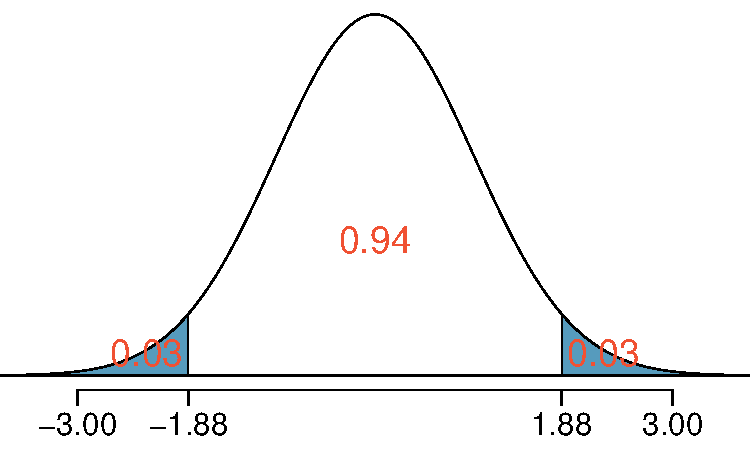
\includegraphics[width=0.4\textwidth]{figures/epilepsy/epilepsy}
\end{center}
\begin{align*}
Z^\star &= 1.88 \\
4 &\ge \frac{1.88 * 18}{\sqrt{n}} \\
n &\ge \left(\frac{1.88 * 18}{4} \right)^2 \\
n &\ge 71.57 \\
&\textit{at least 72}
\end{align*}
\end{multicols}

\vfill

%%%%%%%%%%%%%%%%%%%%%%%%%%%%%%%%%%%%%%%%

\item \qt{Spam} It is estimated that roughly 9\% of incoming email is spam. A spam filter flags 90\% of spam emails as spam, and incorrectly flags 2\% of non-spam emails as spam.


\begin{enumerate}

\item What percent of all email is flagged as spam?

\soln{5cm}{
\begin{align*}
P(flagged~spam) &= P(spam~\&~flagged~spam) + P(not~spam~\&~flagged~spam) \\
&= 0.09 * 0.90 + 0.91 * 0.02 \\
&= 0.081 + 0.0182 \\
&= 0.0992
\end{align*}
}

\item If an email is flagged as spam, what is the probability that it is indeed a spam email?

\soln{5cm}{
\begin{align*}
P(spam~|~flagged~spam) &= \frac{P(spam \& flagged~spam)}{P(flagged~spam)} \\
&= \frac{0.081}{0.0992} \\
&= 0.8165
\end{align*}
}

\end{enumerate}

\vfill

%%%%%%%%%%%%%%%%%%%%%%%%%%%%%%%%%%%%%%%%

\pagebreak

\item \qt{Calcium for treating blood pressure} Lyle et al. (1987) ran an experiment to study the effect of a calcium supplement on the blood pressure of African American males. A group of 10 men received a calcium supplement, and another group of 11 men received a placebo. The experiment lasted 12 weeks. Both before and after the 12-week period, each man had his systolic blood pressure measured while at rest. The changes in blood pressure are given in table below. \\

\begin{center}
\renewcommand{\arraystretch}{1.5}
\begin{tabular}{l | c | c | c | c | c | c | c | c | c | c | c }
Calcium: & -5 	& -4 	& -3 	& -2	&  1 & 7 & 10 & 11 & 17 & 18 \\
\hline
Placebo: & -11 & -5	& -3	&  -3 & -1 &  -1 & -1 &  2 & 3 &  5 &  12 \\
\end{tabular}
\end{center}

$\:$ 

\begin{enumerate}

\item What is the median change in the blood pressure in the \emph{calcium} group?

\soln{3cm}{$Median_{calcium} = \frac{1+7}{2} = 4$}

\item What is the median change in the blood pressure in the \emph{placebo} group?

\soln{3cm}{$Median_{placebo} = -1$}

\item We would like to test if the \emph{median} change in blood pressure is \emph{different} for the calcium and placebo groups. State the hypotheses for this test. 

{\small(\textit{Note:} You can use notation, or you can state your hypotheses in words, but make sure that it's clear what type of test you're doing -- one-sided vs. two-sided.)}

\soln{3cm}{
\begin{align*}
H_0&: Median_{calcium} = Median_{placebo} \\
H_A&: Median_{calcium} \ne Median_{placebo}
\end{align*}
}

\item Calculate the point estimate associated with these hypotheses.

\soln{3cm}{$Median_{calcium} - Median_{placebo} = 5$ \\
}

\pagebreak

\item Since theoretical methods do not apply to sampling distributions of medians, we use a randomization test. To do so, we write the change in blood pressure on 21 index cards. Then, we shuffle these cards and split them into two groups: one group of size 10 representing those receive a calcium supplement, and another group of size 11 representing those on the placebo. We calculate the difference between the medians in the simulated calcium and placebo distributions (as \emph{calcium - placebo}), and record this value. Fill in the blanks in the remainder of this description.

$\:$ 

\begin{adjustwidth}{1.5em}{1.5em}
\begin{doublespace}
We repeat this 100 times to build a randomization distribution, which should be centered at \rule{3cm}{0.5pt}. Lastly, we calculate the p-value as the proportion of simulations where the simulated differences in medians is \rule{3cm}{0.5pt}.
\end{doublespace}
\end{adjustwidth}

\soln{1cm}{0, 5 or more or -5 or less\\
}

\item Calculate the p-value based on the randomization distribution below. Note that the randomization test used 100 simulations.

\[ p-value:  \rule{3cm}{0.5pt} \]

\begin{center}
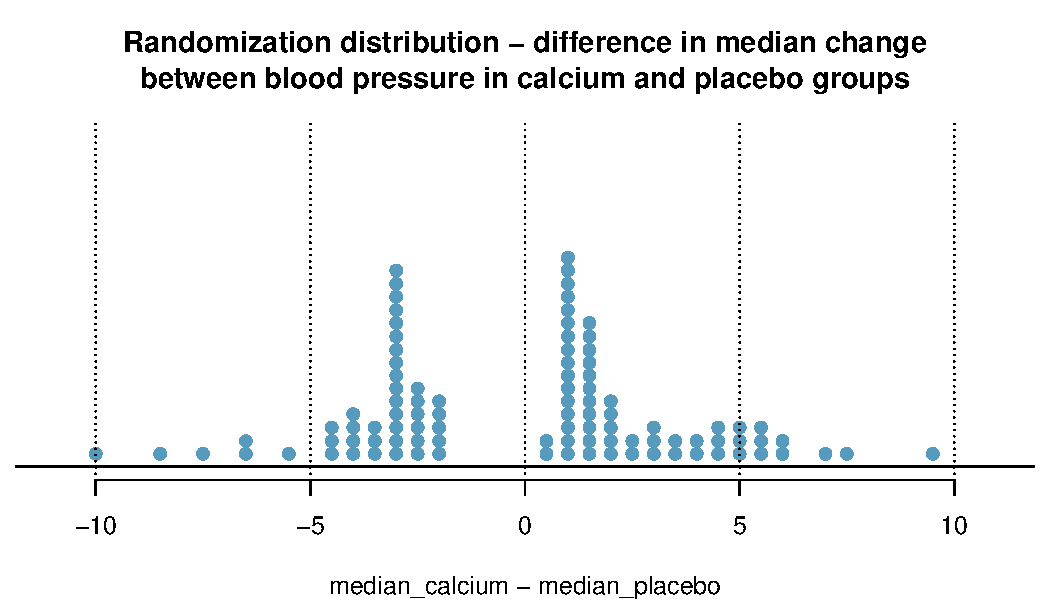
\includegraphics[width=0.8\textwidth]{figures/blood_pressure/blood_pressue_calcium_placebo_randomization.pdf} \vspace{2mm} \\
\end{center}

\soln{0.5cm}{0.17}

\item Refer back to the research question: ``Is there a difference in median change in blood pressure for the calcium and placebo groups?" What does the p-value you calculated in the previous question suggest? Choose one of the following:

\begin{enumerate}[(i)]
\item Reject $H_0$, there is evidence of a difference between the two groups.
\item \solnMult{Fail to reject $H_0$, there isn't sufficient evidence of a difference between the two groups.}
\item Accept $H_0$, there is evidence that the median in the two groups is the same.
\end{enumerate}


\vfill
%

\end{enumerate}

%%%%%%%%%%%%%%%%%%%%%%%%%%%%%%%%%%%%%%%%

\begin{minipage}[b]{0.6\linewidth}
\item \qt{Cats on YouTube} If you randomly select a video on YouTube, the probability that it involves a cat is 0.11. Over the course of a week, you watch 100 videos on YouTube using an app that randomly selects videos (the random video picker). \\

\emph{How many} cat videos would you need to see to suspect that the random video picker is biased towards \emph{or} against cat videos? You can provide a range if need be. \\

\end{minipage}
\begin{minipage}[b]{0.1\linewidth}
\end{minipage}
\begin{minipage}[b]{0.4\linewidth}
\centering
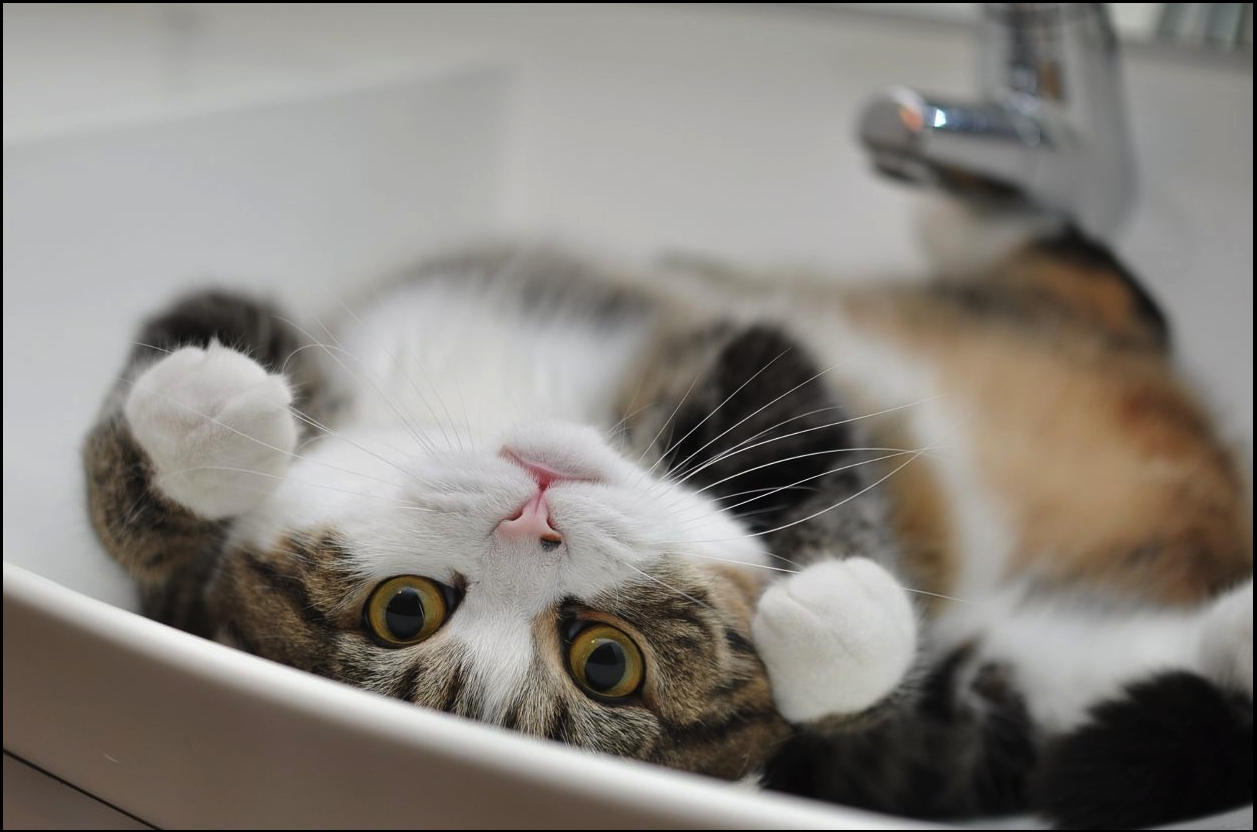
\includegraphics[width=\textwidth]{figures/cat_video/maru}
\end{minipage}
{\small(\textit{Hint:} Think about what would be considered an expected number of videos.)}


\soln{5cm}{
\begin{align*}
\mu &= np = 100 * 0.11 = 11 \\
\sigma &= \sqrt{100 * 0.11 * 0.89} = 3.13 \\
\text{Against: } &11 - (2 * 3.13) =  4.74 \\
\text{Towards: } &11 + (2 * 3.13) = 17.26
\end{align*}
4 or fewer cat videos would indicate bias against, and 18 or more would indicate bias towards.
}

\vfill


%%%%%%%%%%%%%%%%%%%%%%%%%%%%%%%%%%%%%%%%

\pagebreak


\textbf{{\Large Short answer -}} Show your work where necessary.
$\:$ \\


\item  \qt{Help out a friend} An absentminded (and not too clever) scientist friend of yours has just analyzed his data, and he has two numbers -- 26.3 and 2.63 -- written on a scrap of paper. He says: \textit{``I remember that one of these is the standard deviation of my data and the other is the standard error of the mean, but I can�t remember which is which. Can you help?"}

\begin{enumerate}

\item Which number is the standard deviation and which is the standard error of the mean?

\begin{itemize}
\item standard deviation - Circle one:  $\quad$ 26.3 $\quad$2.63
\item[]
\item standard error - Circle one:  $\quad$ 26.3 $\quad$2.63
\item[]
\end{itemize}

\item What was your friend�s sample size?  \rule{2cm}{0.5pt}

\soln{1cm}{n = 100}

\end{enumerate}

\vfill

%

\item \qt{Congress approval amid government shutdown} In a recent Gallup poll on a random sample of 1,028 US adults, 11\% said they approve of the way the Congress is handling its job, with a 95\% confidence interval of 7\% to 15\%. Which of the following statements is/are true based on the confidence interval? Circle \emph{all} that apply. 

(\textit{Note:} To get credit on this question you must circle all of the true statements, and not circle any of the false statements.)\\

\begin{enumerate}[(i)]
\item The population proportion is 0.11.
\item \solnMult{The sample proportion is 0.11.}
\item \solnMult{The margin of error is 0.04.}
\item 95\% of random samples will have sample means between 0.07 and 0.15.
\item \solnMult{It is possible that the population proportion is 0.18.}
\end{enumerate}

\vfill

%

\item \qt{True / False} Determine if the following statements are true or false, and \emph{circle} the appropriate letter (T or F). You do not need to provide your reasoning.

\begin{enumerate}[(i)]

\item (~~T~~/~~F~~) Increasing $\alpha$ increases the power of the test. \tf{T} \\

\item (~~T~~/~~F~~) You are going to collect income data from a right-skewed distribution of incomes of politicians. If you take a large enough sample, the distribution of the incomes of individuals in this sample will be nearly normal. \tf{F} \\

\end{enumerate}

\vfill

%

\pagebreak

\item \qt{Getting past the FDA} Federal guidelines require that pharmaceutical companies provide evidence that a new drug is effective by demonstrating that \emph{two} \emph{independently conducted} randomized studies both show statistically significant benefit from the drug at significance level of 0.025, i.e. $\alpha = 0.025$.

\begin{enumerate}

\item Given that the null hypothesis is that the drug has no benefit, what type of error has been committed if a new drug appears beneficial to the FDA when in fact the drug provides no benefit? Circle one.

\begin{center}
Type 1 $\qquad \qquad$ Type 2 
\end{center}

\soln{0.25cm}{Type 1}

\item If this rule is followed, what is the probability that a new drug will appear beneficial to the FDA when in fact the drug provides no benefit? 
\[ \rule{3cm}{0.5pt} \]

\soln{1.5cm}{$0.025 ^ 2 = 0.000625$}

\end{enumerate}

\vfill
%

\begin{minipage}[c]{0.6\textwidth}
\item \qt{Is sleep necessary?} To investigate, Lesku et al. (2012) measured the activity patterns of breeding pectoral sandpipers (\textit{Calidris melanotos}) in the high Arctic in summer, when the sun never sets. The accompanying figure shows the observed percent time that individual males were awake and active in a 2008 field study. The data are on the left. To the right of the data are the sample mean (filled circle) and error bars for the standard deviation, the standard error of the mean, and a 95\% confidence interval for the mean \emph{in no particular order}.
\end{minipage}
\begin{minipage}[c]{0.1\linewidth}
\end{minipage}
\begin{minipage}[c]{0.3\linewidth}
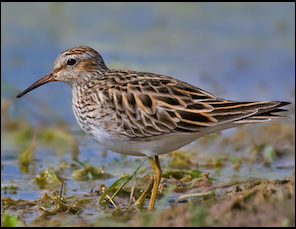
\includegraphics[width=\textwidth]{figures/sleep/sandpiper}
\end{minipage}

\begin{center}
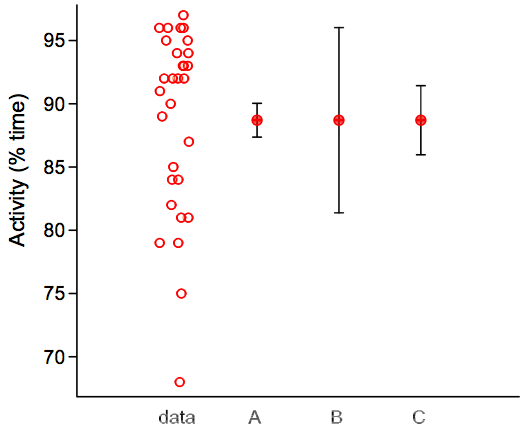
\includegraphics[width=0.5\textwidth]{figures/sleep/sleep}
\end{center}

\begin{adjustwidth}{-1cm}{-1cm}
\begin{enumerate}
\item Which of the error bars indicates the \emph{standard deviation}? Circle one:  $\quad$ A $\quad$ B $\quad$ C \tf{B} \\
\item Which error bar indicates the \emph{standard error} of the mean? Circle one:  $\quad$ A $\quad$ B $\quad$ C \tf{A} \\
\item Which error bar indicates a \emph{95\% confidence interval} for the mean? Circle one:  $\quad$ A $\quad$ B $\quad$ C \tf{C}
\end{enumerate}
\end{adjustwidth}

\vfill
%

%%%%%%%%%%%%%%%%%%%%%%%%%%%%%%%%%%%%%%%%

\pagebreak

\textbf{{\Large Multiple choice -}} Choose the \emph{best} answer. Fill in the bubbles on the first page of the exam. Each question is worth 2 points.  \\

\item Spread of the sampling distribution for the sample mean is mainly determined by the magnitude of the 

\begin{multicols}{2}
\begin{enumerate}
\item sample mean
\item \solnMult{sample size}
\item population mean
\item population size
\item confidence level
\item[]
\end{enumerate}
\end{multicols}

\vfill

%

\item We create multiple sampling distributions, and record the standard error of each. The distributions are for the same point estimate from the same population, but each one is based on a different sample size. For each sampling distribution we record the size of the samples and the standard error of the distribution. The correlation between these two variables will be

\begin{multicols}{2}
\begin{enumerate}
\item zero
\item one
\item \solnMult{negative}
\item positive
\item none of the above
\item[]
\end{enumerate}
\end{multicols}

\vfill

%

\item  A behavioral economist designing an experiment to evaluate people's decision making patterns wants to make sure that males and females are equally represented in the treatment and control groups. Which of the following approaches will be \emph{most} useful?

\begin{multicols}{2}
\begin{enumerate}
\item random sampling
\item random assignment
\item \solnMult{blocking}
\item clustering
\item blinding
\item[]
\end{enumerate}
\end{multicols}

\vfill

%

\pagebreak

\item The Washington Post and the New York Times conducted separate national polls where respondents were asked if they believe congress will reach a deal on the sequester. If the Washington Post surveyed 500 people and reported a 95\% confidence interval while the New York Times surveyed 150 people and reported a 99\% confidence interval. Which paper reported a \emph{larger} margin of error?

\begin{enumerate}
\item The Washington Post
\item \solnMult{The New York Times}
\item The margin of errors are the same. \\
\end{enumerate}

\vfill

%

\item Which of the following is \emph{true}?
\begin{enumerate}
\item Half the observations in a distribution of any shape have positive Z scores.
\item Majority of the values in a right skewed distribution have positive Z scores.
\item \solnMult{An observation with a Z score of $Z = +1.2$ is more unusual than an observation with a Z score of $Z = -0.5$.}
\item The Z score for the median of a distribution of any shape is 0.
\item The median of a left skewed distribution has a negative Z score.
\end{enumerate}

\vfill

\item A research article reports the results of a new drug test. The drug is to be used to decrease symptoms in people with general anxiety disorder (GAD). The article gives a p-value of 0.035 in the analysis section. Which of the interpretations of the p-value is valid?

\begin{choices}
\item The probability that the drug is effective.
\item The probability that the drug is \emph{not} effective.
\item The probability of getting results as extreme as or more extreme than the ones in this study if the drug is actually effective.
\item \solnMult{The probability of getting results as extreme as or more extreme than the ones in this study if the drug is actually \emph{not} effective.}
\end{choices}

\pagebreak
%

\begin{center}
\textit{Answer questions \ref{taxF} to \ref{taxL} based on the information below.}
\end{center}
$\:$
\hrule
$\:$ 

A June Gallup poll asked US residents about their opinion on sales taxes on internet purchases. The results of the poll are summarized in the table below. The text of the survey question is also provided above the table. \\

\begin{center}
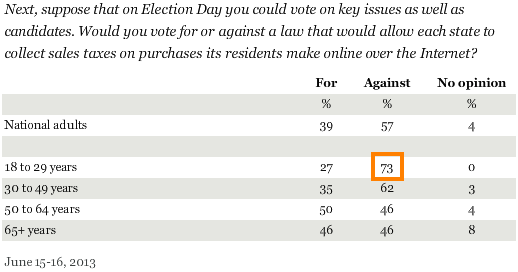
\includegraphics[width=0.7\textwidth]{figures/internet_tax/internet_tax}
\end{center}

$\:$
\hrule
$\:$


\item \label{taxF} One of the values on the table is 73\% (marked). Which of the following best describes this probability?

\begin{enumerate}
\item P(Against)
\item P(18 to 29 years)
\item P(18 to 29 years $|$ Against)
\item \solnMult{P(Against $|$ 18 to 29 years)}
\item P(Against \& 18 to 29 years)
\end{enumerate}

\vfill 

\item \label{taxL} Based on these results, opinion on sales taxes on internet purchases and age appear to be

\begin{enumerate}
\item \solnMult{dependent}
\item independent
\item disjoint
\item mutually exclusive
\item complementary
\end{enumerate}

\vfill

%

\pagebreak

\begin{center}
\textit{Answer questions \ref{boxF} to \ref{boxL} based on the information below.}
\end{center}
$\:$
\hrule
$\:$ 

The two box plots below display distributions of midterm scores for all students in two different sections of a public policy course. \\

\begin{center}
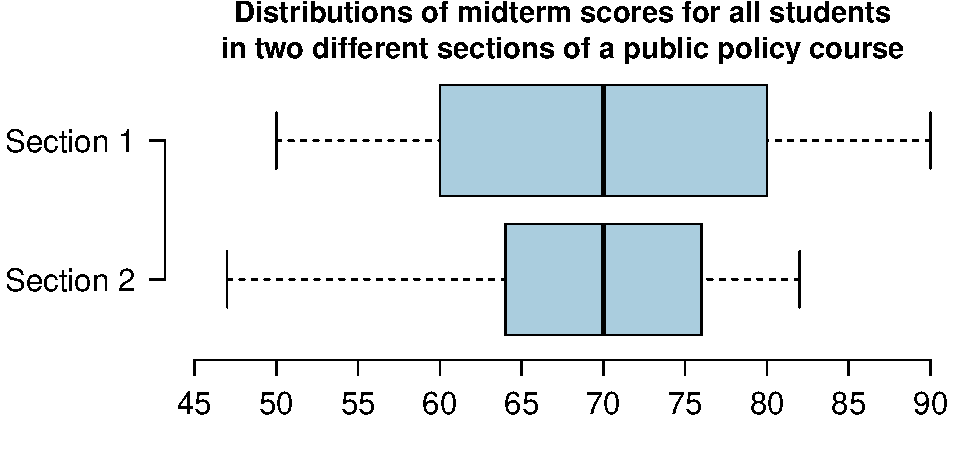
\includegraphics[width=0.7\textwidth]{figures/pubpol_scores/boxplot_mt_score_pubpol_course_sections}
\end{center}

$\:$
\hrule
$\:$

\item \label{boxF} Which section has a greater percentage of students with scores below 55?

\begin{enumerate}
\item Section 1
\item Section 2
\item Both sections are about equal
\item \solnMult{It is impossible to tell}
\end{enumerate}

\vfill

\item Which section has a greater percentage of students with scores above 70?

\begin{enumerate}
\item Section 1
\item Section 2
\item \solnMult{Both sections are about equal}
\item It is impossible to tell
\end{enumerate}

\vfill

%\item \label{boxL} Which section is expected to have a greater standard deviation?
%
%\begin{enumerate}
%\item \solnMult{Section 1}
%\item Section 2
%\item Both sections are about equal
%\item It is impossible to tell
%\end{enumerate}

%
%\vfill
%
%%
%
%\item A research article reports the results of a new drug test. The drug is to be used to decrease symptoms in people with general anxiety disorder (GAD). The article gives a p-value of 0.035 in the analysis section. Which of the interpretations of the p-value is valid?
%
%\begin{choices}
%\item The probability that the drug is effective.
%\item The probability that the drug is \emph{not} effective.
%\item The probability of getting results as extreme as or more extreme than the ones in this study if the drug is actually effective.
%\item \solnMult{The probability of getting results as extreme as or more extreme than the ones in this study if the drug is actually \emph{not} effective.}
%\end{choices}
%
%\vfill
%
%%
%
%\item Suppose half of all newborns are girls and half are boys. Hospital A, a large city hospital, records an average of 50 births a day. Hospital B, a small, rural hospital, records an average of 10 births a day. On a particular day, which hospital is \emph{less likely} to record 80\% or more female births?
%\begin{choices}
%\item \solnMult{Hospital A (with 50 births a day), because the more births you see, the closer the proportions will be to 0.5.}
%\item Hospital B (with 10 births a day), because with fewer births there will be less variability.
%\item The two hospitals are equally likely to record such an event, because the probability of a boy does not depend on the number of births.
%\item This outcome is not possible at either hospital.
%\end{choices}
%
%\vfill
%
%%
%
%\item Each of the 120 students in a statistics class selects a different random sample of 40 quiz scores from a population of 5000 scores they are given. Using their data, each student constructs a 90\% confidence interval for $\mu$, the average quiz score of the
%5000 students. Which of the following conclusions is correct?
%\begin{choices}
%\item About 10\% of the sample means will not be included in the confidence intervals.
%\item \solnMult{About 90\% of the confidence intervals will contain $\mu$.}
%\item It is probable that 90\% of the confidence intervals will be identical.
%\item About 10\% of the raw quiz scores in the samples will not be found in these confidence intervals.
%\end{choices}
%
%\vfill
%
%%
%
%\pagebreak
%
%\item Two polling agencies, Gallup and Public Policy Polling, want to estimate the proportion of American college students who are in favor of same-sex marriage. They both want to have about the same margin of error to estimate this proportion. However, Gallup wants to estimate with 99\% confidence and Public Policy Polling wants to estimate with 95\% confidence. Which agency would need \emph{more} students for their survey in order to obtain the desired margin of error?
%\begin{choices}
%\item \solnMult{Gallup.}
%\item Public Policy Polling.
%\item Both agencies would need the same number of subjects.
%\item It is impossible to obtain the same margin of error with the two different confidence levels.
%\end{choices}
%
%\vfill
%
%%
%
%\item A student participates in a Coke versus Pepsi taste test. She correctly identifies which soda is which four times out of six tries. She claims that this suggests that she can reliably tell the difference between the two soft drinks. You have studied statistics and you want to determine the probability of anyone getting at least four right out of six tries just by chance alone. Which of the following would provide an accurate estimate of that probability?
%\begin{choices}
%\item Have the student repeat this experiment many times and calculate the percentage of times she correctly distinguishes between the brands.
%\item \solnMult{Simulate this on the computer with a 50\% chance of guessing the correct soft drink on each try, and calculate the percent of times there are four or more correct guesses out of six trials.}
%\item Repeat this experiment with a very large sample of people and calculate the percentage of people who make four correct guesses out of six tries.
%\item All of the methods listed above would provide an accurate estimate of the probability.
%\end{choices}
%
%\vfill
%
%%
%
%\item A large university wanted to study the relationship between completing an internship during college and students' future earning potential. From the same graduating class, they selected a random sample of 80 students who completed an internship and 100 students who did not complete an internship and examined their salaries five years after graduation. They found that there was a statistically higher mean salary for the internship group than for the non-internship group. Which of the following interpretations is the \emph{most} appropriate?
%\begin{choices}
%\item More students should complete internships because having an internship produces a higher salary.
%\item \solnMult{There could be a confounding variable, such as student major, that explains the difference in mean salary between the internship and no internship groups.}
%\item You cannot draw any valid conclusions because the sample sizes are different.
%\item We cannot infer anything from these data since the distribution of salaries is likely right skewed.
%\end{choices}
%
%\vfill
%
%%
%
%\pagebreak
%
%%
%
%\item A class of 30 introductory statistics students took a 15 item quiz, with each item worth 1 point. The standard deviation for the resulting score distribution is 0. You know that:
%\begin{choices}
%\item about half of the scores were above the mean
%\item an arithmetic error must have been made
%\item \solnMult{everyone correctly answered the same number of items}
%\item the mean, median, and mode must all be 0
%\end{choices}
%
%\vfill
%
%%
%
%\item Colin, a first-year student, is enrolled in a college algebra course and earned a score of 260 on a math achievement test that was given on to all first-year students prior to enrollment. The instructor looked at two distributions of scores:
%\begin{enumerate}[(1)]
%\item the distribution for all first-year students
%\item the distribution for the first-year students enrolled in this algebra course
%\end{enumerate}
%Both are approximately normally distributed and have the same mean, but the distribution for the algebra course has a smaller standard deviation. 
%
%A Z score is calculated for Colin's test score in both distributions (all first-years and the first-years taking this algebra course). Given that Colin's score is well above the mean, which of the following would be true about these two Z scores?
%\begin{choices}
%\item \solnMult{The Z score based on the distribution for the first-year students taking algebra would be higher.} 
%\item The Z score based on the distribution for all  first-year students would be higher.
%\item The two Z scores would be the same.
%\item The two Z scores would be different, but we don't have enough information to tell which Z score would be higher.
%\end{choices}
%
%\vfill
%
%%
%
%\item A professor gives a test to 120 students and determines the median score. After grading the test, she realizes that the 10 students with the highest scores did exceptionally well. She decides to award these 10 students a bonus of 5 more points.\footnote{Don't get any ideas :)} The median of the new score distribution will be \rule{2cm}{0.5pt} that of the original score distribution.
%\begin{choices}
%\item lower than
%\item \solnMult{equal to}
%\item higher than
%\item depending on skewness, higher or lower than
%\end{choices}
%
%\vfill
%
\end{enumerate}


\pagebreak

\begin{table}[p]
\begin{center}{\small
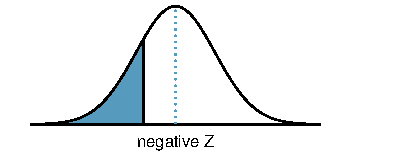
\includegraphics[width=100mm]{figures/normalTails/normalTailLeft} \vspace{2mm} \\
\begin{tabular}{| rrrrr | rrrrr | c}
  \cline{1-10}
&&& \multicolumn{4}{c}{Second decimal place of $Z$} &&& \\
  \cline{1-10}
0.09 &  0.08 &  0.07 &  0.06 &  0.05 &  0.04 &  0.03 &  0.02 &  0.01 &  0.00 & $Z$  \\
  \hline
  \hline
\small{0.0002} & \small{0.0003} & \small{0.0003} & \small{0.0003} & \small{0.0003} & \small{0.0003} & \small{0.0003} & \small{0.0003} & \small{0.0003} & \small{0.0003} & $-3.4$ \\
  \small{0.0003} & \small{0.0004} & \small{0.0004} & \small{0.0004} & \small{0.0004} & \small{0.0004} & \small{0.0004} & \small{0.0005} & \small{0.0005} & \small{0.0005} & $-3.3$ \\
  \small{0.0005} & \small{0.0005} & \small{0.0005} & \small{0.0006} & \small{0.0006} & \small{0.0006} & \small{0.0006} & \small{0.0006} & \small{0.0007} & \small{0.0007} & $-3.2$ \\
  \small{0.0007} & \small{0.0007} & \small{0.0008} & \small{0.0008} & \small{0.0008} & \small{0.0008} & \small{0.0009} & \small{0.0009} & \small{0.0009} & \small{0.0010} & $-3.1$ \\
  \small{0.0010} & \small{0.0010} & \small{0.0011} & \small{0.0011} & \small{0.0011} & \small{0.0012} & \small{0.0012} & \small{0.0013} & \small{0.0013} & \small{0.0013} & $-3.0$ \\
    \hline
    \hline
  \small{0.0014} & \small{0.0014} & \small{0.0015} & \small{0.0015} & \small{0.0016} & \small{0.0016} & \small{0.0017} & \small{0.0018} & \small{0.0018} & \small{0.0019} & $-2.9$ \\
  \small{0.0019} & \small{0.0020} & \small{0.0021} & \small{0.0021} & \small{0.0022} & \small{0.0023} & \small{0.0023} & \small{0.0024} & \small{0.0025} & \small{0.0026} & $-2.8$ \\
  \small{0.0026} & \small{0.0027} & \small{0.0028} & \small{0.0029} & \small{0.0030} & \small{0.0031} & \small{0.0032} & \small{0.0033} & \small{0.0034} & \small{0.0035} & $-2.7$ \\
  \small{0.0036} & \small{0.0037} & \small{0.0038} & \small{0.0039} & \small{0.0040} & \small{0.0041} & \small{0.0043} & \small{0.0044} & \small{0.0045} & \small{0.0047} & $-2.6$ \\
  \small{0.0048} & \small{0.0049} & \small{0.0051} & \small{0.0052} & \small{0.0054} & \small{0.0055} & \small{0.0057} & \small{0.0059} & \small{0.0060} & \small{0.0062} & $-2.5$ \\
    \hline
  \small{0.0064} & \small{0.0066} & \small{0.0068} & \small{0.0069} & \small{0.0071} & \small{0.0073} & \small{0.0075} & \small{0.0078} & \small{0.0080} & \small{0.0082} & $-2.4$ \\
  \small{0.0084} & \small{0.0087} & \small{0.0089} & \small{0.0091} & \small{0.0094} & \small{0.0096} & \small{0.0099} & \small{0.0102} & \small{0.0104} & \small{0.0107} & $-2.3$ \\
  \small{0.0110} & \small{0.0113} & \small{0.0116} & \small{0.0119} & \small{0.0122} & \small{0.0125} & \small{0.0129} & \small{0.0132} & \small{0.0136} & \small{0.0139} & $-2.2$ \\
  \small{0.0143} & \small{0.0146} & \small{0.0150} & \small{0.0154} & \small{0.0158} & \small{0.0162} & \small{0.0166} & \small{0.0170} & \small{0.0174} & \small{0.0179} & $-2.1$ \\
  \small{0.0183} & \small{0.0188} & \small{0.0192} & \small{0.0197} & \small{0.0202} & \small{0.0207} & \small{0.0212} & \small{0.0217} & \small{0.0222} & \small{0.0228} & $-2.0$ \\
    \hline
    \hline
  \small{0.0233} & \small{0.0239} & \small{0.0244} & \small{0.0250} & \small{0.0256} & \small{0.0262} & \small{0.0268} & \small{0.0274} & \small{0.0281} & \small{0.0287} & $-1.9$ \\
  \small{0.0294} & \small{0.0301} & \small{0.0307} & \small{0.0314} & \small{0.0322} & \small{0.0329} & \small{0.0336} & \small{0.0344} & \small{0.0351} & \small{0.0359} & $-1.8$ \\
  \small{0.0367} & \small{0.0375} & \small{0.0384} & \small{0.0392} & \small{0.0401} & \small{0.0409} & \small{0.0418} & \small{0.0427} & \small{0.0436} & \small{0.0446} & $-1.7$ \\
  \small{0.0455} & \small{0.0465} & \small{0.0475} & \small{0.0485} & \small{0.0495} & \small{0.0505} & \small{0.0516} & \small{0.0526} & \small{0.0537} & \small{0.0548} & $-1.6$ \\
  \small{0.0559} & \small{0.0571} & \small{0.0582} & \small{0.0594} & \small{0.0606} & \small{0.0618} & \small{0.0630} & \small{0.0643} & \small{0.0655} & \small{0.0668} & $-1.5$ \\
    \hline
  \small{0.0681} & \small{0.0694} & \small{0.0708} & \small{0.0721} & \small{0.0735} & \small{0.0749} & \small{0.0764} & \small{0.0778} & \small{0.0793} & \small{0.0808} & $-1.4$ \\
  \small{0.0823} & \small{0.0838} & \small{0.0853} & \small{0.0869} & \small{0.0885} & \small{0.0901} & \small{0.0918} & \small{0.0934} & \small{0.0951} & \small{0.0968} & $-1.3$ \\
  \small{0.0985} & \small{0.1003} & \small{0.1020} & \small{0.1038} & \small{0.1056} & \small{0.1075} & \small{0.1093} & \small{0.1112} & \small{0.1131} & \small{0.1151} & $-1.2$ \\
  \small{0.1170} & \small{0.1190} & \small{0.1210} & \small{0.1230} & \small{0.1251} & \small{0.1271} & \small{0.1292} & \small{0.1314} & \small{0.1335} & \small{0.1357} & $-1.1$ \\
  \small{0.1379} & \small{0.1401} & \small{0.1423} & \small{0.1446} & \small{0.1469} & \small{0.1492} & \small{0.1515} & \small{0.1539} & \small{0.1562} & \small{0.1587} & $-1.0$ \\
    \hline
    \hline
  \small{0.1611} & \small{0.1635} & \small{0.1660} & \small{0.1685} & \small{0.1711} & \small{0.1736} & \small{0.1762} & \small{0.1788} & \small{0.1814} & \small{0.1841} & $-0.9$ \\
  \small{0.1867} & \small{0.1894} & \small{0.1922} & \small{0.1949} & \small{0.1977} & \small{0.2005} & \small{0.2033} & \small{0.2061} & \small{0.2090} & \small{0.2119} & $-0.8$ \\
  \small{0.2148} & \small{0.2177} & \small{0.2206} & \small{0.2236} & \small{0.2266} & \small{0.2296} & \small{0.2327} & \small{0.2358} & \small{0.2389} & \small{0.2420} & $-0.7$ \\
  \small{0.2451} & \small{0.2483} & \small{0.2514} & \small{0.2546} & \small{0.2578} & \small{0.2611} & \small{0.2643} & \small{0.2676} & \small{0.2709} & \small{0.2743} & $-0.6$ \\
  \small{0.2776} & \small{0.2810} & \small{0.2843} & \small{0.2877} & \small{0.2912} & \small{0.2946} & \small{0.2981} & \small{0.3015} & \small{0.3050} & \small{0.3085} & $-0.5$ \\
    \hline
  \small{0.3121} & \small{0.3156} & \small{0.3192} & \small{0.3228} & \small{0.3264} & \small{0.3300} & \small{0.3336} & \small{0.3372} & \small{0.3409} & \small{0.3446} & $-0.4$ \\
  \small{0.3483} & \small{0.3520} & \small{0.3557} & \small{0.3594} & \small{0.3632} & \small{0.3669} & \small{0.3707} & \small{0.3745} & \small{0.3783} & \small{0.3821} & $-0.3$ \\
  \small{0.3859} & \small{0.3897} & \small{0.3936} & \small{0.3974} & \small{0.4013} & \small{0.4052} & \small{0.4090} & \small{0.4129} & \small{0.4168} & \small{0.4207} & $-0.2$ \\
  \small{0.4247} & \small{0.4286} & \small{0.4325} & \small{0.4364} & \small{0.4404} & \small{0.4443} & \small{0.4483} & \small{0.4522} & \small{0.4562} & \small{0.4602} & $-0.1$ \\
  \small{0.4641} & \small{0.4681} & \small{0.4721} & \small{0.4761} & \small{0.4801} & \small{0.4840} & \small{0.4880} & \small{0.4920} & \small{0.4960} & \small{0.5000} & $-0.0$ \\
    \hline
\multicolumn{11}{l}{{\normalsize$^*$For $Z \leq -3.50$, the probability is less than or equal to $0.0002$.}}
\end{tabular}}
\end{center}
\end{table}

\begin{table}[p]
\begin{center}{\small
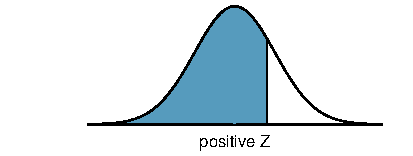
\includegraphics[width=100mm]{figures/normalTails/normalTailRight} \vspace{2mm} \\
\begin{tabular}{c | rrrrr | rrrrr |}
  \cline{2-11}
&&&& \multicolumn{4}{c}{Second decimal place of $Z$} &&& \\
  \cline{2-11}
$Z$ & 0.00 & 0.01 & 0.02 & 0.03 & 0.04 & 0.05 & 0.06 & 0.07 & 0.08 & 0.09 \\
  \hline
  \hline
0.0 & \small{0.5000} & \small{0.5040} & \small{0.5080} & \small{0.5120} & \small{0.5160} & \small{0.5199} & \small{0.5239} & \small{0.5279} & \small{0.5319} & \small{0.5359} \\
  0.1 & \small{0.5398} & \small{0.5438} & \small{0.5478} & \small{0.5517} & \small{0.5557} & \small{0.5596} & \small{0.5636} & \small{0.5675} & \small{0.5714} & \small{0.5753} \\
  0.2 & \small{0.5793} & \small{0.5832} & \small{0.5871} & \small{0.5910} & \small{0.5948} & \small{0.5987} & \small{0.6026} & \small{0.6064} & \small{0.6103} & \small{0.6141} \\
  0.3 & \small{0.6179} & \small{0.6217} & \small{0.6255} & \small{0.6293} & \small{0.6331} & \small{0.6368} & \small{0.6406} & \small{0.6443} & \small{0.6480} & \small{0.6517} \\
  0.4 & \small{0.6554} & \small{0.6591} & \small{0.6628} & \small{0.6664} & \small{0.6700} & \small{0.6736} & \small{0.6772} & \small{0.6808} & \small{0.6844} & \small{0.6879} \\
  \hline
  0.5 & \small{0.6915} & \small{0.6950} & \small{0.6985} & \small{0.7019} & \small{0.7054} & \small{0.7088} & \small{0.7123} & \small{0.7157} & \small{0.7190} & \small{0.7224} \\
  0.6 & \small{0.7257} & \small{0.7291} & \small{0.7324} & \small{0.7357} & \small{0.7389} & \small{0.7422} & \small{0.7454} & \small{0.7486} & \small{0.7517} & \small{0.7549} \\
  0.7 & \small{0.7580} & \small{0.7611} & \small{0.7642} & \small{0.7673} & \small{0.7704} & \small{0.7734} & \small{0.7764} & \small{0.7794} & \small{0.7823} & \small{0.7852} \\
  0.8 & \small{0.7881} & \small{0.7910} & \small{0.7939} & \small{0.7967} & \small{0.7995} & \small{0.8023} & \small{0.8051} & \small{0.8078} & \small{0.8106} & \small{0.8133} \\
  0.9 & \small{0.8159} & \small{0.8186} & \small{0.8212} & \small{0.8238} & \small{0.8264} & \small{0.8289} & \small{0.8315} & \small{0.8340} & \small{0.8365} & \small{0.8389} \\
  \hline
  \hline
  1.0 & \small{0.8413} & \small{0.8438} & \small{0.8461} & \small{0.8485} & \small{0.8508} & \small{0.8531} & \small{0.8554} & \small{0.8577} & \small{0.8599} & \small{0.8621} \\
  1.1 & \small{0.8643} & \small{0.8665} & \small{0.8686} & \small{0.8708} & \small{0.8729} & \small{0.8749} & \small{0.8770} & \small{0.8790} & \small{0.8810} & \small{0.8830} \\
  1.2 & \small{0.8849} & \small{0.8869} & \small{0.8888} & \small{0.8907} & \small{0.8925} & \small{0.8944} & \small{0.8962} & \small{0.8980} & \small{0.8997} & \small{0.9015} \\
  1.3 & \small{0.9032} & \small{0.9049} & \small{0.9066} & \small{0.9082} & \small{0.9099} & \small{0.9115} & \small{0.9131} & \small{0.9147} & \small{0.9162} & \small{0.9177} \\
  1.4 & \small{0.9192} & \small{0.9207} & \small{0.9222} & \small{0.9236} & \small{0.9251} & \small{0.9265} & \small{0.9279} & \small{0.9292} & \small{0.9306} & \small{0.9319} \\
  \hline
  1.5 & \small{0.9332} & \small{0.9345} & \small{0.9357} & \small{0.9370} & \small{0.9382} & \small{0.9394} & \small{0.9406} & \small{0.9418} & \small{0.9429} & \small{0.9441} \\
  1.6 & \small{0.9452} & \small{0.9463} & \small{0.9474} & \small{0.9484} & \small{0.9495} & \small{0.9505} & \small{0.9515} & \small{0.9525} & \small{0.9535} & \small{0.9545} \\
  1.7 & \small{0.9554} & \small{0.9564} & \small{0.9573} & \small{0.9582} & \small{0.9591} & \small{0.9599} & \small{0.9608} & \small{0.9616} & \small{0.9625} & \small{0.9633} \\
  1.8 & \small{0.9641} & \small{0.9649} & \small{0.9656} & \small{0.9664} & \small{0.9671} & \small{0.9678} & \small{0.9686} & \small{0.9693} & \small{0.9699} & \small{0.9706} \\
  1.9 & \small{0.9713} & \small{0.9719} & \small{0.9726} & \small{0.9732} & \small{0.9738} & \small{0.9744} & \small{0.9750} & \small{0.9756} & \small{0.9761} & \small{0.9767} \\
  \hline
  \hline
  2.0 & \small{0.9772} & \small{0.9778} & \small{0.9783} & \small{0.9788} & \small{0.9793} & \small{0.9798} & \small{0.9803} & \small{0.9808} & \small{0.9812} & \small{0.9817} \\
  2.1 & \small{0.9821} & \small{0.9826} & \small{0.9830} & \small{0.9834} & \small{0.9838} & \small{0.9842} & \small{0.9846} & \small{0.9850} & \small{0.9854} & \small{0.9857} \\
  2.2 & \small{0.9861} & \small{0.9864} & \small{0.9868} & \small{0.9871} & \small{0.9875} & \small{0.9878} & \small{0.9881} & \small{0.9884} & \small{0.9887} & \small{0.9890} \\
  2.3 & \small{0.9893} & \small{0.9896} & \small{0.9898} & \small{0.9901} & \small{0.9904} & \small{0.9906} & \small{0.9909} & \small{0.9911} & \small{0.9913} & \small{0.9916} \\
  2.4 & \small{0.9918} & \small{0.9920} & \small{0.9922} & \small{0.9925} & \small{0.9927} & \small{0.9929} & \small{0.9931} & \small{0.9932} & \small{0.9934} & \small{0.9936} \\
  \hline
  2.5 & \small{0.9938} & \small{0.9940} & \small{0.9941} & \small{0.9943} & \small{0.9945} & \small{0.9946} & \small{0.9948} & \small{0.9949} & \small{0.9951} & \small{0.9952} \\
  2.6 & \small{0.9953} & \small{0.9955} & \small{0.9956} & \small{0.9957} & \small{0.9959} & \small{0.9960} & \small{0.9961} & \small{0.9962} & \small{0.9963} & \small{0.9964} \\
  2.7 & \small{0.9965} & \small{0.9966} & \small{0.9967} & \small{0.9968} & \small{0.9969} & \small{0.9970} & \small{0.9971} & \small{0.9972} & \small{0.9973} & \small{0.9974} \\
  2.8 & \small{0.9974} & \small{0.9975} & \small{0.9976} & \small{0.9977} & \small{0.9977} & \small{0.9978} & \small{0.9979} & \small{0.9979} & \small{0.9980} & \small{0.9981} \\
  2.9 & \small{0.9981} & \small{0.9982} & \small{0.9982} & \small{0.9983} & \small{0.9984} & \small{0.9984} & \small{0.9985} & \small{0.9985} & \small{0.9986} & \small{0.9986} \\
  \hline
  \hline
  3.0 & \small{0.9987} & \small{0.9987} & \small{0.9987} & \small{0.9988} & \small{0.9988} & \small{0.9989} & \small{0.9989} & \small{0.9989} & \small{0.9990} & \small{0.9990} \\
  3.1 & \small{0.9990} & \small{0.9991} & \small{0.9991} & \small{0.9991} & \small{0.9992} & \small{0.9992} & \small{0.9992} & \small{0.9992} & \small{0.9993} & \small{0.9993} \\
  3.2 & \small{0.9993} & \small{0.9993} & \small{0.9994} & \small{0.9994} & \small{0.9994} & \small{0.9994} & \small{0.9994} & \small{0.9995} & \small{0.9995} & \small{0.9995} \\
  3.3 & \small{0.9995} & \small{0.9995} & \small{0.9995} & \small{0.9996} & \small{0.9996} & \small{0.9996} & \small{0.9996} & \small{0.9996} & \small{0.9996} & \small{0.9997} \\
  3.4 & \small{0.9997} & \small{0.9997} & \small{0.9997} & \small{0.9997} & \small{0.9997} & \small{0.9997} & \small{0.9997} & \small{0.9997} & \small{0.9997} & \small{0.9998} \\
   \hline
\multicolumn{11}{l}{{\normalsize$^*$For $Z \geq 3.50$, the probability is greater than or equal to $0.9998$.}}
\end{tabular}}
\end{center}
\end{table}

\end{document}